\documentclass[abstracton,12pt]{scrartcl}
    
\usepackage[utf8]{inputenc}
% \usepackage[T1]{fontenc}
\usepackage{fancyhdr}
\usepackage{graphicx}
\usepackage{tikz}
\usepackage{listings}
\usepackage{amssymb}
\usepackage{amsfonts}
\usepackage{amsmath}
\usepackage{amsthm}
\usepackage{pdfpages}
\usepackage{forest}
\usepackage{multicol}
\usepackage{varwidth}
\usepackage{verbatim}
\usepackage{cleveref}
\usepackage{minted}
\usepackage[ruled,vlined]{algorithm2e}
\usepackage{caption}
\usepackage{subcaption}
\usepackage{soul}
\usepackage{microtype}
\usepackage{pgfplots}
% \usepackage{ulem}
% \usepackage{ifthen}
% \usepackage{wrapfig}
% \usepackage{geometry}
% \usepackage{titlesec}

\forestset{qtree/.style={for tree={parent anchor=south, child anchor=north,align=left,inner sep=0pt}}}
\graphicspath{ {images/} }
\pgfplotsset{yticklabel style={text width=2.5em,align=right}}
% \setlength{\multicolsep}{6.0pt plus 2.0pt minus 1.5pt}% 50% of original values
% \titleformat{\chapter}{}{\thechapter}{}{}
% \titlespacing{\chapter}{-100pt}{-100pt}{-100pt}

% --------- 

\titlehead{Department of Informatics, University of Zürich}
\subject{\vspace*{2cm}MSc Basismodul}
\title{The Adaptive Radix Tree}
\author{
    Rafael Kallis\\[-5pt]
    \scriptsize Matrikelnummer: 14-708-887\\[-5pt]
    \scriptsize Email: \texttt{rk@rafaelkallis.com}
}
\date{\vspace*{2cm}September 1, 2018}
\publishers{
    \small supervised by Prof.\ Dr.\ Michael\ Böhlen and Kevin\ Wellenzohn \\[5cm]
    \begin{tikzpicture}[overlay]
    \node at (-3,-3) {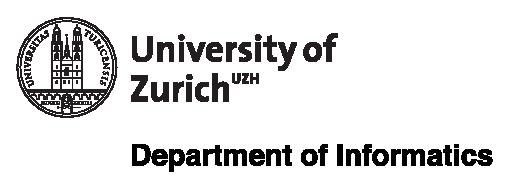
\includegraphics[height=1.5cm]{IFIlogo}};
    \node at (7,-3) {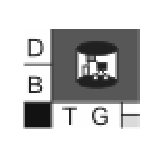
\includegraphics[height=1.5cm]{dbtgBW}};
    \end{tikzpicture}
}

% \dedication{dedicated to xxx}

% --------- 

\theoremstyle{definition}

\newtheorem{definition}{Definition}
% \newtheorem{figure}{Figure}
\newtheorem{example}{Example}
% \newtheorem{theorem}{Theorem}
% \newtheorem{lemma}{Lemma}

\crefname{algocfline}{algorithm}{algorithms}
\Crefname{algocfline}{Algorithm}{Algorithms}

\crefname{figure}{Fig.}{Figs.}
\Crefname{figure}{Figure}{Figures}

\crefname{example}{Ex.}{Ex.}
\Crefname{example}{Example}{Examples}

% \newenvironment{proof}
%     {\noindent{\bf Proof:\rm}}{\hfill$\Box$\vspace{\medskipamount}}

\newenvironment{centerverbatim}{\par\centering\varwidth{\linewidth}\verbatim}
    {\endverbatim\endvarwidth\par}

\def\bbbr{{\rm I\!R}}
\def\bbbm{{\rm I\!M}}
\def\bbbn{{\rm I\!N}}
\def\bbbz{{\rm I\!Z}}

% --------- 

\begin{document}

\maketitle

% \chapter*{Acknowledgements}

% \begin{abstract}
%   ...
% \end{abstract}

% \chapter*{Zusammenfassung}

% \tableofcontents
% \listoffigures
% \listoftables

\newpage
\section{Introduction}

Main-Memory Databases increasingly become a viable option for many applications
due to the considerably faster access times and increasing capacities of 
volatile memory in comparison to secondary storage.

Leis et al.\ \cite{leis2013adaptive} propose the Adaptive Radix Tree (ART), an in-memory
data structure which efficiently stores and retrieves data.
As we will see later, ART achieves its performance, and space
efficiency, by compressing the tree both vertically and horizontally.

The goal of this project is to study and implement ART, as proposed by 
\cite{leis2013adaptive}. 
In \Cref{sec:art} we describe how ART is constructed by applying 
vertical and horizontal compression to a trie.
Next, we describe the point query procedure, as well as 
key deletion in \Cref{sec:algorithms}.
Finally, a benchmark of ART, a red-black tree and a hashtable
is presented in \Cref{sec:benchmarks}.

\section{Preliminaries}\label{sec:preliminaries}

A trie \cite{fredkin1960trie} is a hierarchical data structure which
stores key-value pairs. Tries can answer both point and range queries 
efficiently since keys are stored in lexicographic order.
Unlike a comparison-based search tree, a trie does not store keys in nodes.
Rather, the digital representation of a search key is split into partial
keys used to index the nodes. When 
constructing a trie from a set of keys, all insertion orders result in the 
same tree. Tries do not require rebalancing operations and therefore have 
no notion of balance, unlike comparison based search trees.

Keys are split into partial keys of $s$ bits, where $s$ is called 
\textit{span}. Inner nodes have  $2^s$ child pointers 
(possibly \texttt{null}), one for each possible $s$-bit sequence. During tree
traversal, we descend down to the child node identified by the $d$-th
$s$-bit partial key of the search key, where $d$ is the depth of the current 
node.  Using an array of $2^s$  pointers, this lookup can be done without any 
additional comparison. 

\Cref{fig:span} depicts tries storing the 
8-bit keys ``$01000011$'', ``$01000110$'' and ``$01100100$'' with 
$s \in \{1,2\}$. Span $s$ is critical for the performance of the trie because $s$ 
determines the height of the trie. We observe that by increasing the span, 
we decrease the tree height. A trie
storing $k$ bit keys has $\lceil \frac{k}{s} \rceil$ levels of nodes.
As a consequence, point queries, insertions and deletions have 
$O(k)$ complexity.

Span $s$ also determines the space consumption of the tree.
A node with span $s$ requires $2^s$ pointers. 
An apparent trade off exists between tree height versus space efficiency that
depends on $s$. Increasing $s$ yields a decrease in the tree's height, 
resulting in faster lookups because less nodes are traversed. On the other
hand, by increasing $s$, nodes require to store more child pointers. Every
increment in $s$ halves the height of the tree but (nearly) doubles the space consumed
by each node.

\begin{figure}[h]
  \centering
  \begin{subfigure}[b]{0.4\textwidth}
    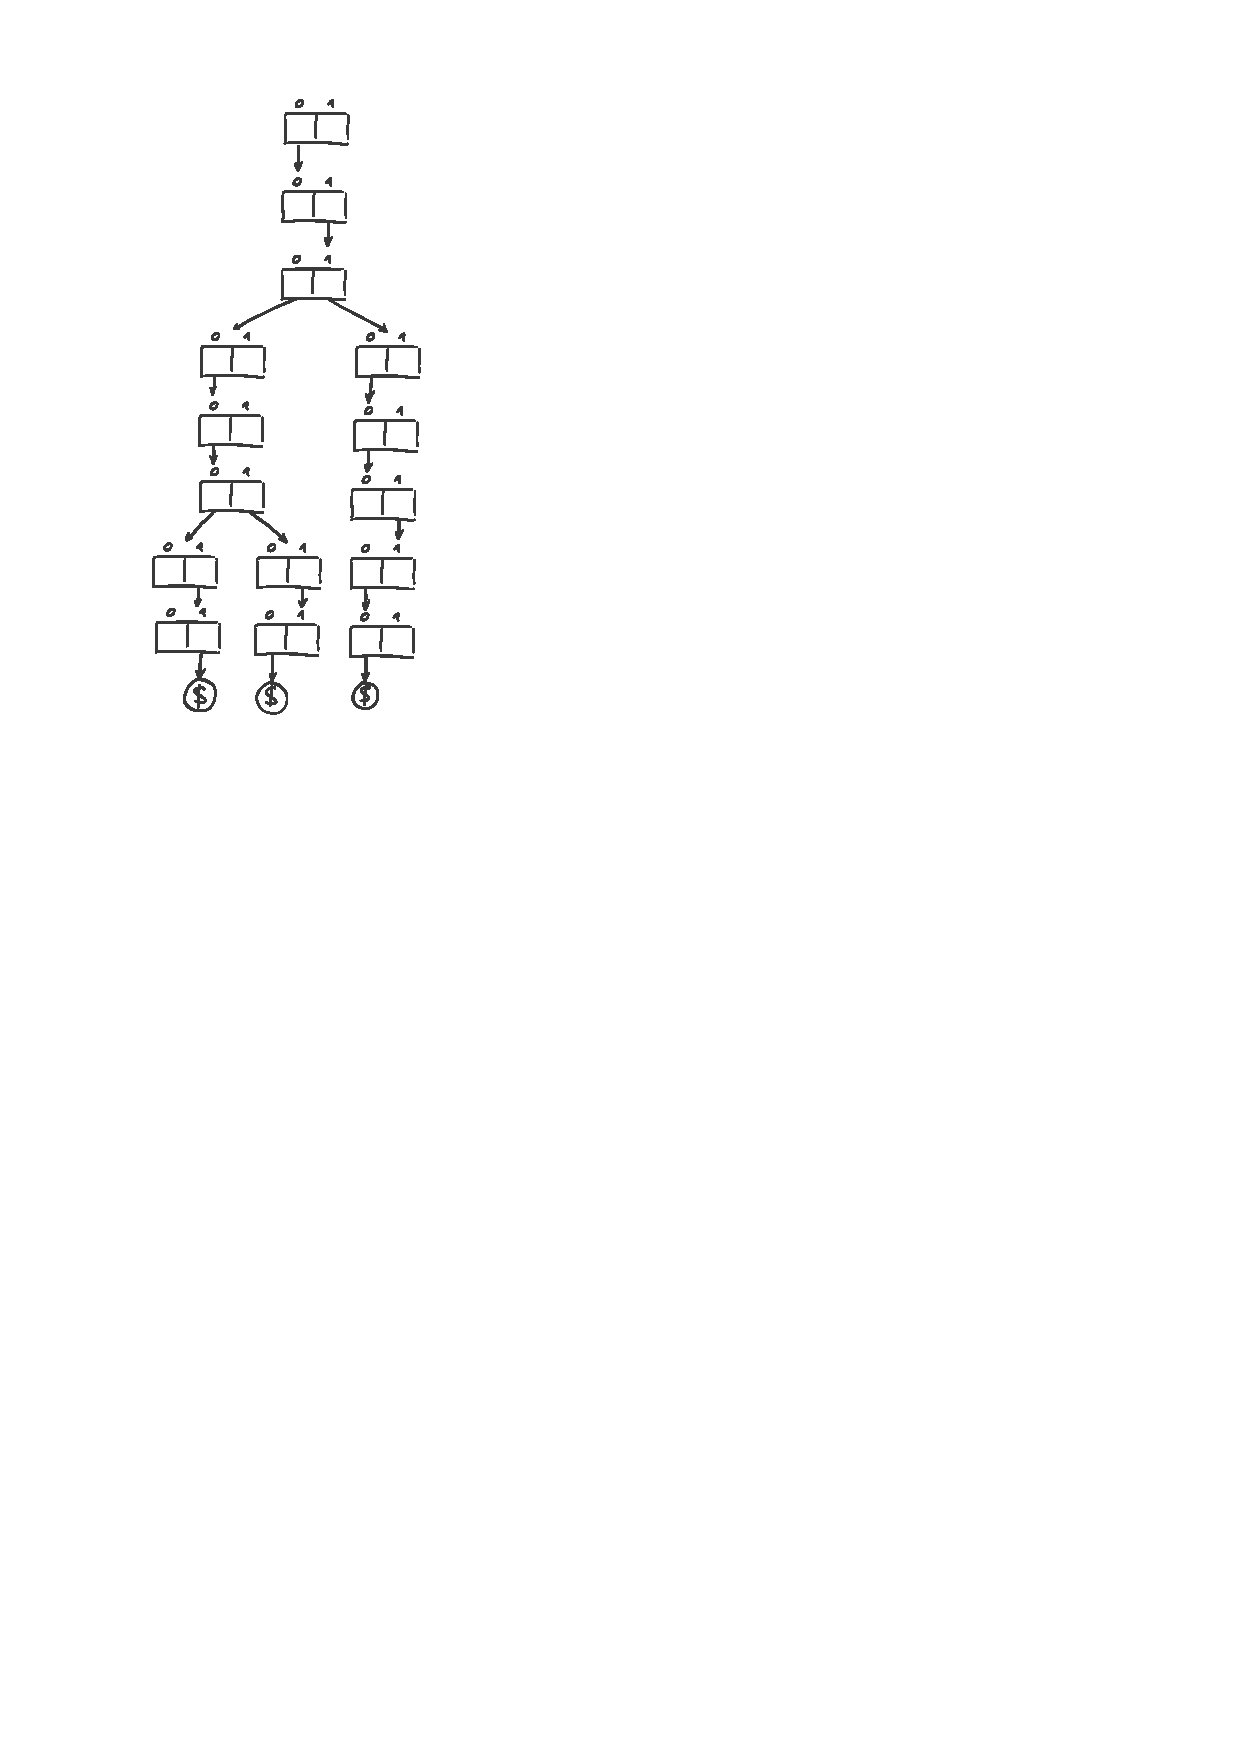
\includegraphics[height=10cm,trim={2cm 17.5cm 2.5cm 1.5cm},clip]{trie_s1_draw}
    \caption{$s=1$}
  \end{subfigure}
  \begin{subfigure}[b]{0.55\textwidth}
    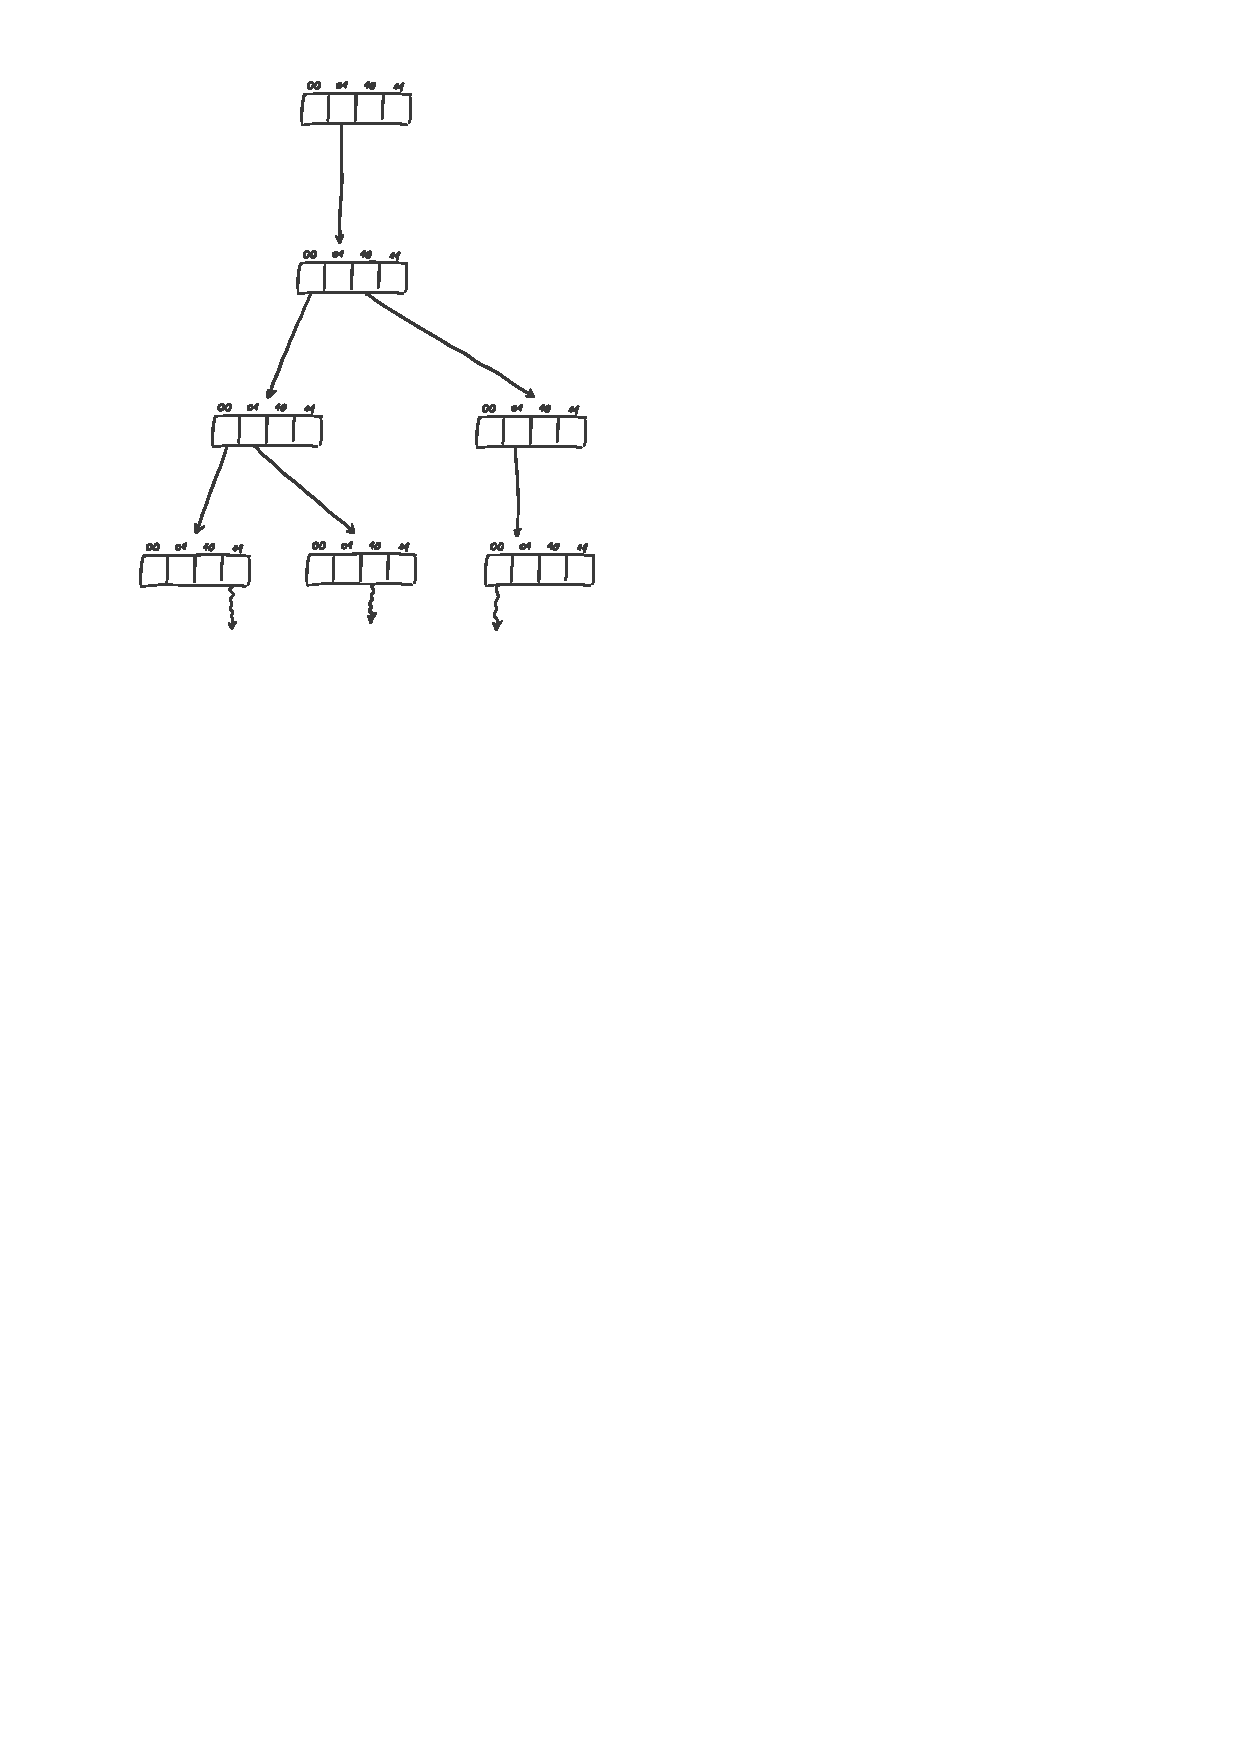
\includegraphics[height=10cm,trim={2cm 18.5cm 2.5cm 0.5cm},clip]{trie_s2_draw}
    \caption{$s=2$}
  \end{subfigure}
  \caption{
    Tries with span $s \in \{1,2\}$ storing keys ``$01000011$'', ``$01000110$''
    and ``$01100100$''.
  }
  \label{fig:span}
\end{figure}

\newpage

\section{Adaptive Radix Tree (ART)}\label{sec:art}

The \textit{Adaptive Radix Tree} (ART) is a space efficient trie, which
achieves its low memory consumption using \textit{vertical} and 
\textit{horizontal} compression. Using vertical compression, ART reduces
the tree height significantly by merging parent nodes with child nodes
under certain circumstances. Horizontal compression reduces the amount
of space required by each node depending on the number of child nodes.

\subsection{Vertical (Prefix) Compression}\label{sec:vertical-compression}

When storing long keys, chains of nodes start to form where each node only
has a single child. (e.g.\ the trie in \Cref{fig:span} stores ``01100100'',
we see a chain of five nodes).
As a consequence, a lot of space is wasted as many nodes
with little actual content are kept and traversals are slowed down because
many nodes are traversed. Space wasting is further amplified with sparse
datasets or a small span.

Morrison introduced \textit{Patricia}~\cite{morrison1968patricia}. 
Patricia is a space-optimized trie in which
each node with no siblings is merged with its parent, i.e.\ inner nodes
are only created if they are required to distinguish at least two leaf nodes. 
Doing so, chains caused by long keys are eliminated, which make tries 
space-inefficient. Although Morrison's Patricia tree is a bitwise trie, i.e.\ 
has a span $s=1$, the technique can be applied to tries with any span,
although it becomes less effective as span $s$ increases.
We refer to this technique as \textit{vertical compression}.

Leis et al.\ mention three approaches to deal with vertical compression:
\begin{itemize}
  \item Pessimistic: We store an additional variable, called \texttt{prefix},
    inside each node. This variable stores the concatenation of partial keys
    of descendants that were eliminated because they had no siblings. During
    lookup, \texttt{prefix} is compared to the search key before preceding to
    the next child. \Cref{fig:vertical-compression} depicts two tries, one 
    with and one without vertical compression. We observe that nodes with no 
    siblings, color coded red, are eliminated and their partial key is 
    appended to the parent's prefix.

  \item Optimistic: Only the number of compressed nodes is stored. Lookups
    just skip this number of partial keys without comparing them to the search
    key. Keys are required to be stored on leaf nodes. When a lookup arrives
    to a leaf node, its key must be compared to the search key. 

  \item Hybrid: We store the number of compressed nodes and a static array
    in order to store a part of the compressed path. If the number of
    compressed nodes exceeds the size of the array, the optimistic strategy is
    used instead.
\end{itemize}

\begin{figure}[h]
  \begin{footnotesize}
    \begin{multicols}{2}
      \noindent
      \begin{flushright}
      \framebox(160,160){
        \begin{forest}
          [,circle,draw
            [,circle,draw,red, edge label={node[midway,right,font=\footnotesize]{$01$}}
              [,circle,draw, edge label={node[midway,left,font=\footnotesize]{$00$}}
                [,circle,draw, edge label={node[midway,left,font=\footnotesize]{$00$}}
                  [,circle,draw,red, edge label={node[midway,left,font=\footnotesize]{$11$}}]
                ]
                [,phantom]
                [,circle,draw, edge label={node[midway,right,font=\footnotesize]{$01$}}
                  [,circle,draw,red, edge label={node[midway,right,font=\footnotesize]{$10$}}]
                ]
              ]
              [,phantom]
              [,phantom]
              [,circle,draw, edge label={node[midway,right,font=\footnotesize]{$10$}}
                [,circle,draw,red, edge label={node[midway,right,font=\footnotesize]{$01$}}
                  [,circle,draw,red, edge label={node[midway,right,font=\footnotesize]{$00$}}]
                ]
              ]
            ]
          ]
        \end{forest}
      }
      \hspace{5mm}
      \end{flushright}
      ~

      \begin{flushleft}
      \hspace{5mm}
      \framebox(160,160){
        \begin{forest}
          [,circle,draw
            [,circle,draw, edge label={node[midway,left,font=\footnotesize]{$00$}}
              [,circle,draw, edge label={node[midway,left,font=\footnotesize]{$00$}}]{
                \draw[gray] (.east)--++(0.5em,0em)
                  node[anchor=west,gray]{11};
              }
              [,phantom]
              [,circle,draw, edge label={node[midway,right,font=\footnotesize]{$01$}}]{
                \draw[gray] (.east)--++(0.5em,0em)
                  node[anchor=west,gray]{10};
              }
            ]
            [,phantom]
            [,phantom]
            [,circle,draw, edge label={node[midway,right,font=\footnotesize]{$10$}}]{
              \draw[gray] (.east)--++(0.5em,0em)
                node[anchor=west,gray]{0100};
            }
          ]{
            \draw[gray] (.east)--++(0.5em,0em)
              node[anchor=west,gray]{01};
          }
        \end{forest}
      }
      \end{flushleft}
    \end{multicols}
  \end{footnotesize}
  \caption{
    Tries with span $s=2$ storing keys ``$01000011$'', ``$01000110$''
    and ``$01100100$''. The trie on the right incorporates (pessimistic)
    vertical compression. Red nodes indicate nodes which get eliminated under
    vertical compression. Gray strings represent the value of the prefix 
    variable.
  }
  \label{fig:vertical-compression}
\end{figure}

\newpage

\subsection{Horizontal Compression (Adaptive Nodes)}\label{sec:horizontal-compression}

With large values of span $s$, an excessive amount of space is sacrificed
to achieve a smaller tree height. Space is allocated for pointers which keep
references to child nodes, even if they are unused.

In order to reduce the space needed to keep
such references, Leis et al.\ propose \textit{Adaptive Nodes} 
\cite{leis2013adaptive}, which make use of dynamic data structures 
instead of static arrays for child node bookkeeping. Doing so, we allocate 
less space when the number of children is small and add more 
space if required, i.e.\ more children are added.
We refer to this technique as \textit{horizontal compression}.
Leis et al.\ fix the span $s=8$, i.e. partial keys are 1 byte
long and therefore each node can have up to $2^8 = 256$ children.

When applying horizontal compression, a node is in one of four configurations, 
depending on the number of child nodes. Each of the four configurations is 
optimized for a different amount of children.
When keys are inserted/deleted, the nodes are adapted accordingly.
The most compact configuration 
is called \texttt{Node4} which can carry up to four children. 
In the same manner, we also have \texttt{Node16}, \texttt{Node48} 
and \texttt{Node256}. All nodes have a header which stores the node type,
the number of children and the prefix variable, which contains the compressed
path (c.f.\ \Cref{sec:vertical-compression}).

\begin{table}[h]
  \centering
  \begin{tabular}{ l|r|r } 
    Type & Children & Space (bytes) \\
    \hline
    \texttt{Node4} & 2-4 & $h + 4 + 4 \cdot 8 = h + 36$ \\ 
    \texttt{Node16} & 5-16 & $h + 16 + 16 \cdot 8 = h + 144$ \\ 
    \texttt{Node48} & 17-48 & $h + 256 + 48 \cdot 8 = h + 640$ \\ 
    \texttt{Node256} & 49-256 & $h + 256 \cdot 8 = h + 2048$ 
  \end{tabular}
  \caption{Space consumption for each inner node type. $h$ is equal to
    the size of the header.}
  \label{tbl:node-sizes}
\end{table}

We now describe the structure of each of the four configurations.
\Cref{tbl:node-sizes} shows the space consumption for each inner node type.
Note that $h$ is equal to the header's size.
\Cref{fig:horizontal-compression} illustrates the state of a node
for each node type, when storing the partial keys $65$ (``01000001''), 
$82$ (``01010010''), $84$ (``01010100'') and pointers to their corresponding 
child nodes $\alpha$, $\beta$, $\gamma$. Note that $\varnothing$ represents 
a \texttt{null} pointer.

A node of type \texttt{Node4} contains two 4-element arrays, one called
``partial keys'' and one called ``children''.
The ``partial keys'' array, holds
partial keys which identify children of that node. 
The ``children'' array, holds pointers to the child nodes.
Partial keys and pointers are stored at corresponding positions in their
respective arrays and the partial keys are sorted.

A node of type \texttt{Node16} is structured similarly
to \texttt{Node4}, the only difference being the lengths of the two static 
arrays, which are 16 each.

An instance of \texttt{Node48} contains a 256-element array named 
``indexes'' and a 48-element array called ``children''.
Partial keys are stored implicitly in ``indexes'', i.e.\ 
can be indexed with partial key bytes directly.
As the name suggests, ``indexes'' stores the index of a child
node inside the ``children'' array.

Finally, a node of type \texttt{Node256} contains an array of
256 pointers which can be indexed with partial key bytes directly.
Child nodes can be found with a single lookup.

\begin{figure}[H]
  \centering
  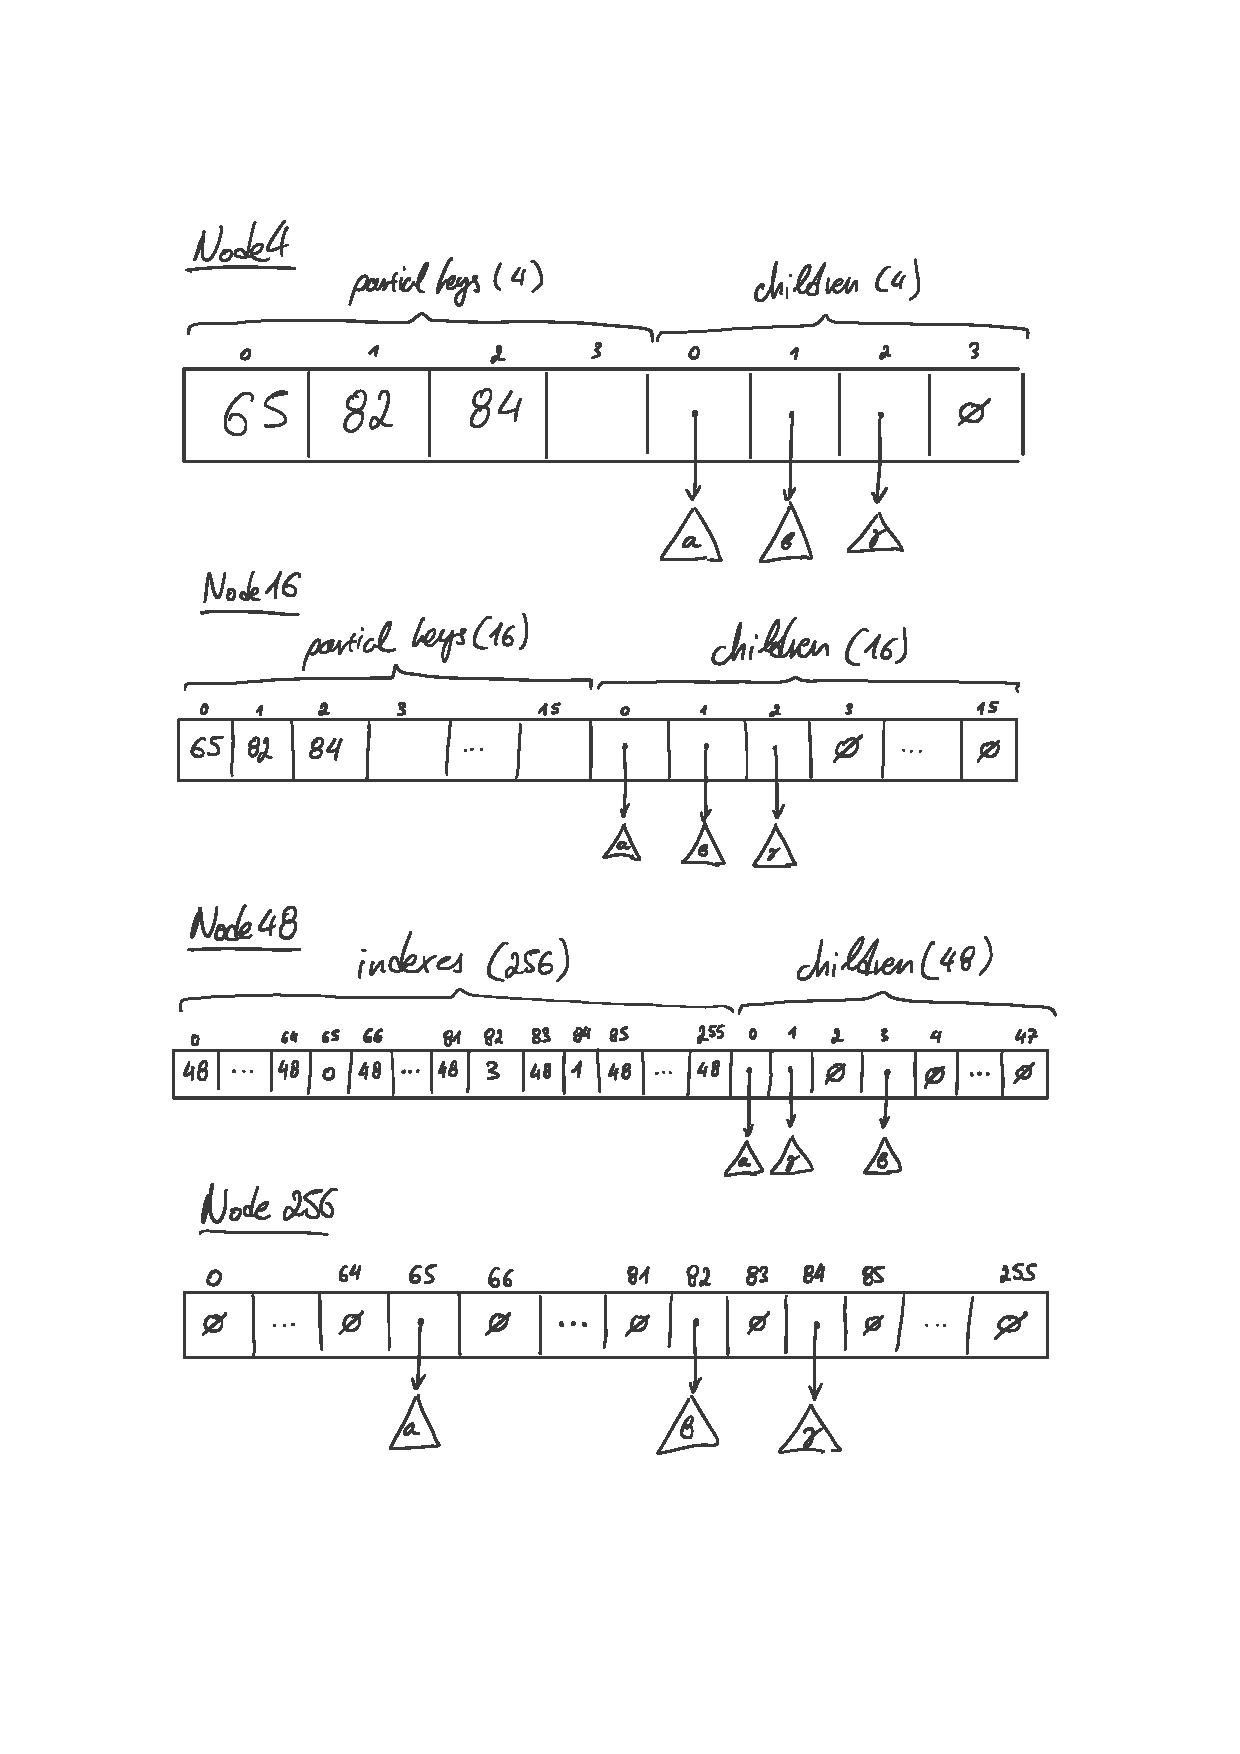
\includegraphics[height=20cm,trim={2.5cm 5cm 2.5cm 3.5cm},clip]{art_nodes_draw}
  \caption{
    When horizontal compression is applied, a node is in one of four 
    configurations, namely \texttt{Node4}, \texttt{Node16}, \texttt{Node48} 
    and \texttt{Node256}.
    Each of the four configurations is optimized for a different number of 
    child nodes. We store the partial keys $65$, $82$, $84$ and their 
    corresponding child nodes $\alpha$, $\beta$, $\gamma$ in an instance
    of each node type. Note that $\varnothing$ represents a \texttt{null} 
    pointer.
  }
 \label{fig:horizontal-compression}
\end{figure}

\newpage

\section{Algorithms}\label{sec:algorithms}

\vspace{-1mm}
We will now describe how two fundamental operations, namely
point query and deletion are implemented in ART.
Range queries and insertions are similar and are omitted for brevity.
The algorithms mentioned below are based on the implementations presented by
Leis et al. 

Note that our implementation uses
\textit{single-value leaves} (c.f.\ Leis et al.), 
i.e.\ values are stored using an additional leaf node type, conveniently
called \texttt{Node0}, which stores one value. Additionally, we utilize
pessimistic vertical compression (c.f.\ \Cref{sec:vertical-compression}),
i.e.\ each inner node stores the entire compressed path inside the 
\texttt{prefix} variable using a variable length partial key array. 
We present our implementations below.

\vspace{-3mm}
\subsection{Point Query}\label{sec:point-query}

The code fragment in \Cref{algo:point-query} shows the implementation of a 
point query on ART in C++. Method \texttt{get} accepts a key and its length
as an argument and returns a pointer to the value associated with the given 
key, or \texttt{null} if the key is not found.

In lines 2-3 we declare and initialize a pointer, \texttt{cur}, which references
the current node during tree traversal, \texttt{child} which references 
\texttt{cur}'s child and \texttt{depth}, which holds the depth
of the current node. We now enter a loop in which we check if \texttt{cur} 
references \texttt{null} during the beginning of each iteration, and if so, 
we return \texttt{null}.

In lines 5-8 we check if a prefix mismatch occurs. This step is required
because of vertical compression (c.f.\ \Cref{sec:vertical-compression}).
Method \texttt{check\_prefix} is a member of the \texttt{node} class which
determines the number of matching bytes between \texttt{cur}'s prefix
and \texttt{key} w.r.t.\ the current depth. If a prefix mismatch is discovered,
\texttt{null} is returned.

Lines 9-12 check for an exact match of the key at the current node. If so,
we return the value of the current node.

Finally, we traverse to the next child node. \texttt{depth} is increased to
account for the nodes merged due to vertical compression.
We lookup the next child node, which is assigned to \texttt{cur}.
If no such child exists, the search key does not exist and \texttt{null} is
returned.

\begin{figure}[H]
  \begin{minted}[numbers=left,frame=single,fontsize=\scriptsize]{c++}
template <class T> T * art<T>::get(const char *key, const int key_len) const {
  node<T> *cur = root_, **child = nullptr;
  int depth = 0;
  while (cur != nullptr) {
    if (cur->prefix_len_ != cur->check_prefix(key + depth, key_len - depth)) {
      /* prefix mismatch */
      return nullptr;
    }
    if (cur->prefix_len_ == key_len - depth) {
      /* exact match */
      return cur->value_;
    }
    child = cur->find_child(key[depth + cur->prefix_len_]);
    cur = child != nullptr ? *child : nullptr;
    depth += cur->prefix_len_ + 1;
  }
  return nullptr;
}
  \end{minted}
  \vspace{-5mm}
  \caption{Point query implemented in C++.}
  \label{algo:point-query}
\end{figure}

\subsection{Deletion}\label{sec:deletion}

\Cref{algo:deletion} presents our implementation of key deletion on ART in C++.
During deletion, the leaf node is removed from an inner node, which is shrunk
if necessary. If the leaf to remove only has one sibling, vertical
compression is applied. We assume all leaf nodes are of type \texttt{Node0}.

In lines 3-5, we declare and initialize two pointers, \texttt{cur} and
\texttt{par} which reference the current and parent node during tree traversal.
Variable \texttt{cur\_partial\_key} holds the partial key which indexes the
current node in the parent's child lookup table.
Variable \texttt{depth} holds the depth of the current node.

Next, we loop until \texttt{cur} references either the right leaf node or
\texttt{null}. For the latter, \texttt{null} is returned.

Line 12 checks if \texttt{cur} is a leaf node, i.e.\ the node that contains 
the search key has been found. If that is not the case, we
continue descending down (lines 57-60). Given \texttt{cur} is a leaf, one
of three cases is possible depending on \texttt{cur}'s siblings:

\begin{itemize}
  \item If \texttt{cur} has \textit{no siblings} (lines 18-24), \texttt{cur}
    must be the root. We delete \texttt{cur} and set the root to \texttt{null}.

  \item If \texttt{cur} has \textit{one sibling} (lines 24-48), vertical
    compression is applied, effectively removing both \texttt{cur} and its
    parent \texttt{par}. During this process, \texttt{par}'s \texttt{prefix},
    as well as the sibling's partial key, are prepended to the sibling's
    \texttt{prefix}.

  \item If \texttt{cur} has \textit{more than one sibling} (lines 48-54),
    we simply remove \texttt{cur} from its parent \texttt{par} and shrink
    \texttt{par} if needed (c.f.\ \Cref{sec:horizontal-compression}).
\end{itemize}

Finally, the value associated with the search key is returned (in case the
method callee has to free resources).

\begin{figure}[H]
  \begin{minted}[numbers=left,frame=single,fontsize=\scriptsize]{c++}
template <class T> T *art<T>::del(const char *key, const int key_len) {
  if (root_ == nullptr) { return nullptr; }
  node<T> **par = nullptr, **cur = &root_;
  char cur_partial_key;
  int depth = 0;

  while (cur != nullptr) {
    if ((**cur).prefix_len_ != (**cur).check_prefix(key + depth, key_len - depth)) {
      /* prefix mismatch */
      return nullptr;
    }
    if (key_len == depth + (**cur).prefix_len_) {
      /* exact match */
      T *value = (**cur).value_;
      (**cur).value_ = nullptr;
      int n_siblings = par != nullptr ? (**par).n_children() - 1 : 0;

      if (n_siblings == 0) {
        /* cur is root */
        if ((**cur).prefix_ != nullptr) { delete[](**cur).prefix_; }
        delete (*cur);
        *cur = nullptr;

      } else if (n_siblings == 1) {
        /* find sibling and apply vertical compression */
        char sibling_partial_key = (**par).next_partial_key(0);
        if (sibling_partial_key == cur_partial_key) {
          sibling_partial_key = (**par).next_partial_key(cur_partial_key + 1);
        }
        node<T> *sibling = *(**par).find_child(sibling_partial_key);
        char *old_prefix = sibling->prefix_;
        int old_prefix_len = sibling->prefix_len_;
        /* compute new prefix of sibling */
        sibling->prefix_ = new char[(**par).prefix_len_ + 1 + old_prefix_len];
        sibling->prefix_len_ = (**par).prefix_len_ + 1 + old_prefix_len;
        std::memcpy(sibling->prefix_, (**par).prefix_, (**par).prefix_len_);
        sibling->prefix_[(**par).prefix_len_] = sibling_partial_key;
        std::memcpy(sibling->prefix_ + (**par).prefix_len_ + 1, old_prefix,
               old_prefix_len);
        if (old_prefix != nullptr) { delete[] old_prefix; }
        /* remove cur and par */
        if ((**cur).prefix_ != nullptr) { delete[](**cur).prefix_; }
        delete (*cur);
        if ((**par).prefix_ != nullptr) { delete[](**par).prefix_; }
        delete (*par);
        *par = sibling;

      } else if (n_siblings > 1) {
        /* remove cur */
        if ((**cur).prefix_ != nullptr) { delete[](**cur).prefix_; }
        delete (*cur);
        (**par).del_child(cur_partial_key);
        if ((**par).is_underfull()) { *par = (**par).shrink(); }
      }
      return value;
    }
    cur_partial_key = key[depth + (**cur).prefix_len_];
    depth += (**cur).prefix_len_ + 1;
    par = cur;
    cur = (**cur).find_child(cur_partial_key);
  }
  return nullptr;
}
  \end{minted}
  \caption{Key deletion implemented in C++.}
 \label{algo:deletion}
\end{figure}

\newpage

\section{Benchmarks}\label{sec:benchmarks}

% \vspace{-2mm}
In this section we compare the performance of ART against the two text book
data structures red-black tree (RBT) and chained hash table (HT).
We chose RBT to compete against ART because, like ART, RBT is a hierarchical
data structure with sorted keys, and supports answering both point and range
queries efficiently. HT do answer point queries faster but lack support for
efficient range queries. We use C++ standard library containers 
\texttt{std::map} and \texttt{std::unordered\_map}\footnote{https://en.cppreference.com/w/cpp/container}
which are implementations of RBT and HT, respectively.
We would like to see ART outperforming RBT but do not expect ART performing
better than HT. 

We first conduct a series of microbenchmarks in order to assess lookup,
insertion and deletion performance. Then we run a mixed workload benchmark
on the three data structures and finally we conduct an experiment in order
to measure how often vertical compression is applied on ART. There are two 
datasets, i.e.\ set of keys, used for the benchmarks, a sparse
and a dense dataset. A set of keys is dense (sparse) if many (few) members
share common prefixes.

\vspace{-3mm}
\subsection{Microbenchmarks}\label{sec:microbenchmarks}

% \vspace{-1mm}
During the lookup microbenchmark, we execute point queries on an instance
of each of the three data structures (ART, RBT, HT)
containing the same four million keys. The keys are sparse (i.e.\ uniformly
distributed), 64-bit integers. Each key is queried exactly once.
The insertion microbenchmark inserts the same four million sparse 64-bit keys
used previously. Finally, the deletion microbenchmark, structured similar to 
the lookup microbenchmark, attempts to delete every stored key from the data 
structure.

\Cref{fig:lookup-microbenchmark,fig:insertion-microbenchmark,fig:deletion-microbenchmark}
show the results of the three microbenchmarks. ART is positioned in between 
its competitors in all three microbenchmarks.

\begin{figure}[H]
  \centering
  \begin{subfigure}[b]{0.3\textwidth}
    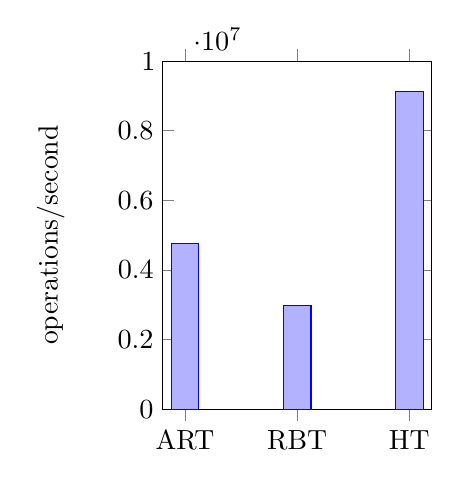
\begin{tikzpicture}
      \begin{axis}[
        ybar,
        symbolic x coords={ART,RBT,HT},
        ylabel=operations/second,
        ymax = 10000000,
        ymin = 0,
        width=5cm,
        height=6cm,
        ]
        \addplot coordinates {(ART,4770407.4) (RBT,2977984.9) (HT,9121391.1)};
      \end{axis}
    \end{tikzpicture}
    \caption{Lookup}
    \label{fig:lookup-microbenchmark}
  \end{subfigure}
  \begin{subfigure}[b]{0.3\textwidth}
    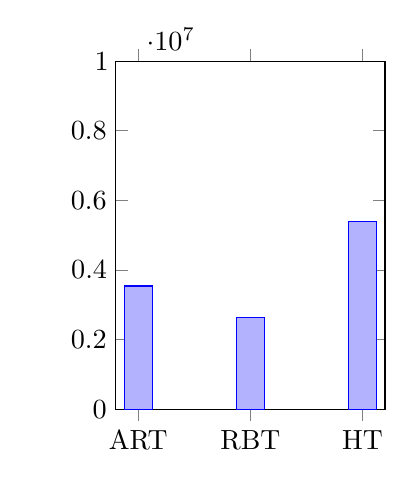
\begin{tikzpicture}
      \begin{axis}[
        ybar,
        symbolic x coords={ART,RBT,HT},
        ymax = 10000000,
        ymin = 0,
        width=5cm,
        height=6cm,
        ]
        \addplot coordinates {(ART,3537978.9) (RBT,2642926.8) (HT,5384934.8)};
      \end{axis}
    \end{tikzpicture}
    \caption{Insertion}
    \label{fig:insertion-microbenchmark}
  \end{subfigure}
  \begin{subfigure}[b]{0.3\textwidth}
    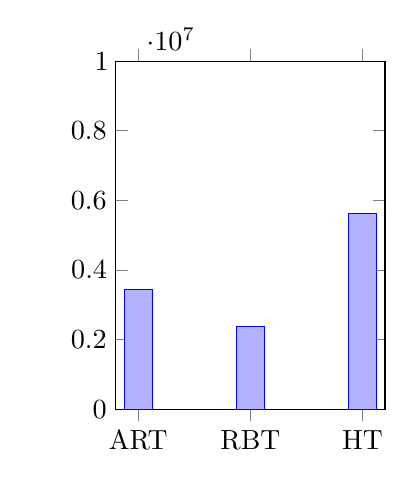
\begin{tikzpicture}
      \begin{axis}[
        ybar,
        symbolic x coords={ART,RBT,HT},
        ymax = 10000000,
        ymin = 0,
        width=5cm,
        height=6cm,
        ]
        \addplot coordinates {(ART,3430847.9) (RBT,2362525.6) (HT,5610399.1)};
      \end{axis}
    \end{tikzpicture}
    \caption{Deletion}
    \label{fig:deletion-microbenchmark}
  \end{subfigure}
  \caption{Lookup, insertion and deletion performance of ART,
  red-black trees (RBT) and hashtables (HT).}
  \label{fig:microbenchmark}
\end{figure}

\subsection{Main Benchmark}
\label{sec:main-benchmark}

We now conduct a benchmark which assesses the transactional throughput of 
a well defined workload applied on each of the three data structures.

The more than twelve million keys used during the benchmark have structure
and do resemble paths of a hierarchy (e.g.\ ``\texttt{/a}'', ``\texttt{/a/b}'',
``\texttt{/a/c}'', etc.). The dataset is based on DELL's 
website~\cite{wellenzohn2017wapi}.
The keys are ordered in reverse level order and during each transaction we
draw a key under the Zipf distribution (skew $s=1$).

We query against the randomly drawn key, and if the query returns no results,
i.e.\ the key does not exist, we insert the key, otherwise we delete it.
Transactions are executed in sequential order.

As \Cref{fig:main-benchmark} shows, ART performs as good as RBT and HT clearly
outperforms its competitors.

\begin{figure}[H]
  \centering
  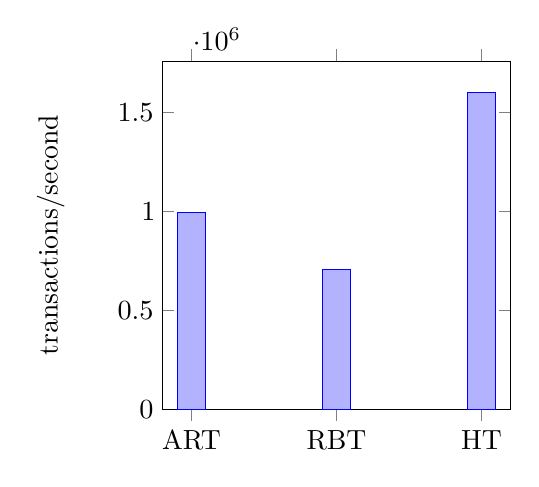
\begin{tikzpicture}
    \begin{axis}[
      ybar,
      symbolic x coords={ART,RBT,HT},
      ylabel=transactions/second,
      ymin=0,
      width=6cm,
      height=6cm,
      ]
      \addplot coordinates {(ART,995467.8) (RBT,704264.2) (HT,1598781.4)};
    \end{axis}
  \end{tikzpicture}
  \caption{Transactional throughput of ART,
    red-black trees and hashtables over a skewed workload with
    mixed reads and writes.}
  \label{fig:main-benchmark}
\end{figure}

\subsection{Vertical Compression}
\label{sec:compression-benchmark}

Our last experiment measures how often vertical compression is applied.
As mentioned in \Cref{sec:vertical-compression} when deleting a node with
a single sibling, the sibling is compressed, i.e.\ merged with its parent.

If each transaction only deletes one existing key, the number of compressions
cannot exceed the number of transactions. The number of compressions
depends on span $s$. If $s=1$, every node must have exactly one sibling,
and therefore every deletion requires a compression, unless the root is
deleted. ART has a span of $s=8$ and we therefore do not expect a compression 
for every deletion.

Results should also vary depending if keys are sparse or dense. Dense keys
likely share common prefixes and as a result tries require less nodes to 
store the keys. We expect that having dense keys imply smaller number
of compressions due to the smaller number of nodes.

\Cref{fig:compressions-sparse,fig:compressions-dense} depict number of vertical
compressions over number of transactions for sparse and dense keys. 
We observe a linear relation between the two variables. As expected, 
dense keys require less compressions compared to sparse keys. That is because 
less nodes are needed to store dense keys, thus path compression is applied
fewer times.

\begin{figure}[H]
  \centering
  \begin{subfigure}[b]{0.49\textwidth}
    \begin{tikzpicture}
      \begin{axis}[
        xmax=11000000,
        ymax=4500000,
        xlabel=transactions,
        ylabel=\#compressions,
        height=7cm,
        width=7cm,
        ]
        \addplot table {compressions_sparse.dat};
      \end{axis}
    \end{tikzpicture}
    \caption{Sparse Keys}
    \label{fig:compressions-sparse}
  \end{subfigure}
  \begin{subfigure}[b]{0.49\textwidth}
    \begin{tikzpicture}
      \begin{axis}[
        xmax=11000000,
        ymax=4500000,
        xlabel=transactions,
        ylabel=\#compressions,
        height=7cm,
        width=7cm,
        ]
        \addplot table {compressions_paths.dat};
      \end{axis}
    \end{tikzpicture}
    \caption{Dense Keys}
    \label{fig:compressions-dense}
  \end{subfigure}
  \caption{Number of compressions over number of transactions. Each transaction
  deletes a random key.}
\end{figure}

\vspace{-5mm}
\section{Future Work}
\label{sec:future-work}

In this project we implemented all basic functionalities of ART, but left 
potential for performance improvements.

Our implementation uses C++ dynamic arrays, i.e. \texttt{std::vector} in order
to store compressed paths, which requires $24 + n$ bytes, where $n$ is the
number of compressed nodes. Using C-style arrays, nodes require only $12 + n$
bytes to support vertical compression.

We also plan to optimize commonly used procedures, e.g.\ prefix checking
against a search key or child node lookup/modification by leveraging the vastly
faster C++ standard library array comparison and modification methods
(e.g.\ \texttt{memcmp}, \texttt{memset}) and try avoiding loops.

Leis et al.\ use \textit{hybrid} vertical compression, i.e.\ only store the
8 first bytes of the compressed path in a static array and the number of
compressed nodes. We use pessimistic vertical compression, which stores
the entire compressed path.
Their approach leverages on-CPU caches since it decreases memory fragmentation
but keys must be stored at the leaves and one additional comparison is
required at the leaf node. We want to know how strong we benefit from hybrid 
vertical compression and how much it impacts memory consumption.

Finally, our implementation dictates single threaded usage, but we intend to
incorporate concurrency control in order to further increase the transactional
throughput of ART when multiple cores are present.

\newpage

\bibliographystyle{abbrv}
\bibliography{art}

\end{document}
